\sf\Large

%\centerline{\LARGE\bf РЕАЛЬНЫЕ ГАЗЫ}
До сих пор мы говорили об {\bf идеальном газе}: молекулы -- это твердые шарики, соударяющиеся упруго. Размерами пренебрегаем. Взаимодействие -- только в момент удара.

Однако, мы знаем, что при больших давлениях законы Бойля-Мариотта и Гей-Люссака не работают. Причины очевидны:
\begin{enumerate}
\item Молекулы -- не точечные; в формулах надо учитывать их размеры, которые при большом давлении занимают существенную долю объема.
\item Молекулы -- не твердые шарики; силы взаимодействия между ними имеют сложный характер.
\end{enumerate}
 \begin{picture}(185,35)(0,0)
 %\put(0,0){\framebox(185,35)[b]{}}
 \put(10,0){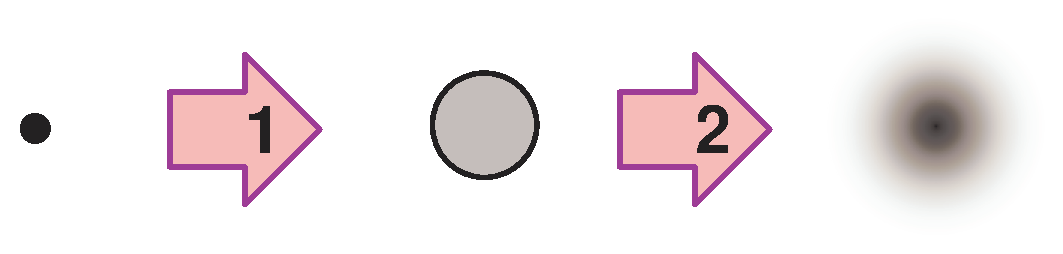
\includegraphics{GP011/GP011F01.eps}}
 %\put(0,0){\makebox(0,0)[tl]{\parbox{125mm}{}}}
 \end{picture}\\

 Ван-дер-Ваальс (Johannes Diderik van der Waals, 1837 - 1923, Amsterdam) все это учел.
Для идеального газа было
\begin{displaymath}
pV_0=RT
\end{displaymath}
1) Если считать суммарный объем всех молекул равным $b$, то получится, что эффективный простор, в котором могут метаться молекулы, меньше реального объема газа на эту величину, и уравнение преображается:
\begin{displaymath}
p(V_0-b)=RT
\end{displaymath}
2) На большом расстоянии молекулы слегка притягиваются друг к другу, и газ немного сжимается, как если бы давление было повыше -- не $p$, а $p+p_i$, где $p_i$ -- некое ``внутреннее'' давление. Итого, имеем
\begin{displaymath}
(p+p_i)(V_0-b)=RT
\end{displaymath}
Осталось как-то определить величину этих поправок. Сначала определимся с величиной $b$. Пусть в объеме есть только 2 молекулы с радиусом $r$ и объемом $v=\frac43\pi r^3$. Какой объем недоступен для их движения? Ответ: центры молекул не могут сблизиться меньше чем на $2r$. То есть, на двоих недоступен объем $\frac43\pi (2r)^3=8v$, а на одну молекулу -- $4v$. Итак, поправка $b$ примерно равна учетверенному суммарному объему всех молекул.

Если с поправкой $b$ все ясно, то с ``внутренним давлением'' все сложнее.
 
 \begin{picture}(185,30)(0,0)
 %\put(0,0){\framebox(185,30)[b]{}}
 \put(145,0){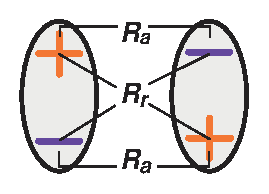
\includegraphics{GP011/GP011F02.eps}}
 \put(0,28){\makebox(0,0)[tl]{\parbox{140mm}{
В целом, молекулы нейтральны и кулоновски притягиваться не могут. Но зато могут поляризоваться! Причина при\-тя\-же\-ния -- в поляризации.
Действительно: при дан\-ном расположении диполей, расстояние между }}}
 \end{picture}\\
разноименными зарядами меньше, чем между одноименными ($R_A<R_r$), и поскольку силы как притяжения, так и отталкивания, $\sim 1/R^2$, то на небольших расстояниях притяжение пересиливает. Если считать, что {\bf каж\-дый} из N диполей, находящихся в некотором рассматриваемом объеме, взаимодействует с {\bf каждым} из остальных N--1, то количество притягива\-ю\-щих связей
=N(N--1). При большом N это превращается в $\simeq$N$^2$. Таким образом, вторая поправка, связанная с притяжением молекул, должна быть $\sim$ квадрату числа молекул в единице объема $\sim n_0^2$ или обратно пропорциональна квадрату молярного объема $\sim1/V_0^2$.

Итак, уравнение Ван-дер-Ваальса:
\begin{equation}
\left(p+\frac{a}{V_0^2}\right)\left(V_0-b\right)=RT
\end{equation}
Если у нас не 1 моль газа, а, например, некая масса $m$, то занимаемый газом объем $V$ будет в $m/\mu$ раз больше: $V=V_0\cdot m/\mu$. Выразив отсюда $V_0$ через $V$, подставим его в уравнение:
\begin{equation}
\left(p+\frac{m^2}{\mu^2}\frac{a}{V^2}\right)\left(V-\frac{m}{\mu}b\right)=\frac{m}{\mu}RT
\end{equation}
 \begin{picture}(185,42)(0,0)
 %\put(0,0){\framebox(185,40)[b]{}}
 \put(55,0){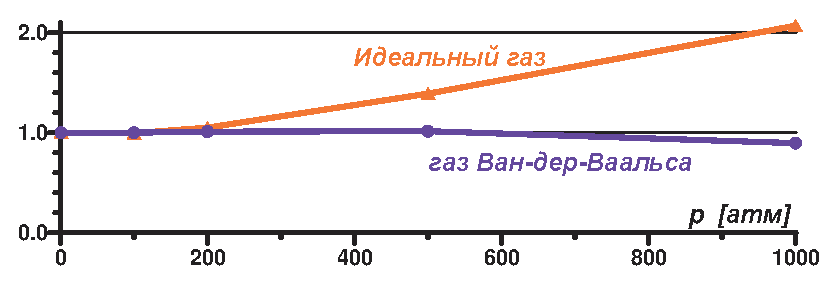
\includegraphics{GP011/GP011F04.eps}}
 \put(0,38){\makebox(0,0)[tl]{\parbox{50mm}{
Это выполняется уже гораздо лучше, чем уравнение для идеальных газов, но все же не точно.
 }}}
 \end{picture}\\
 \begin{picture}(185,75)(0,0)
 %\put(0,0){\framebox(185,75)[b]{}}
 \put(15,0){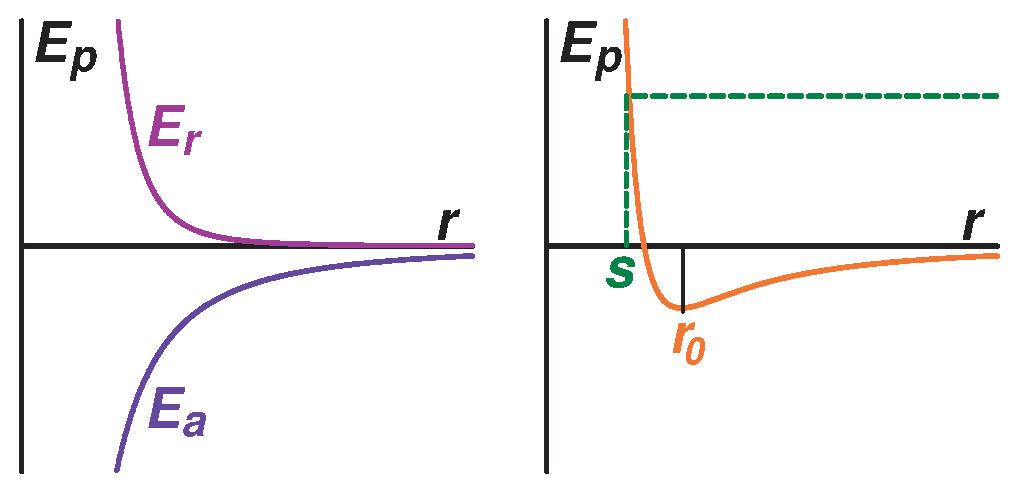
\includegraphics{GP011/GP011F03.eps}}
 \put(0,38){\makebox(0,0)[tl]{\parbox{50mm}{
 }}}
 \end{picture}\\
Силы между молекулами: отталкивание ($f_{\rm repulsion}$) и притяжение ($f_{\rm attraction}$). Потенциальная энергия $E_r>0$ и $E_a<0$. Притяжение с расстоянием убывает медленнее, зато отталкивание при $r\rightarrow0$ растет круче.

Объяснение: как уже говорилось, молекулы издали слегка притяги\-ва\-ют\-ся друг к другу из-за поляризации. Вблизи же, когда их электронные оболочки соприко\-с\-ну\-лись, начинается резкое кулоновское отталкивание ядер, т.к. оболочки их (ядра) больше не экранируют.

В итоге имеем характерную кривую с минимумом при $r=r_0$. Если бы у молекул не было кинетической энергии, то они бы расположились на $r_0$ друг от друга и так в этих потенциальных ямах и сидели бы. На самом же деле, имея какую-то $E_k>0$, соответствующую данной температуре, они сближаются, немного даже разгоняясь из-за притяжения (пунктир обозначает уровень ПОЛНОЙ энергии $E=E_p+E_k$). При $r<r_0$ молекулы ``проскакивают'' точку равновесия, начинают тормозиться и совсем оста\-на\-в\-ли\-ваются при $r=s$ (это максимально возможное сближение), а затем снова разлетаются.\\
 \begin{picture}(185,45)(0,0)
 %\put(0,0){\framebox(185,45)[b]{}}
 \put(15,20){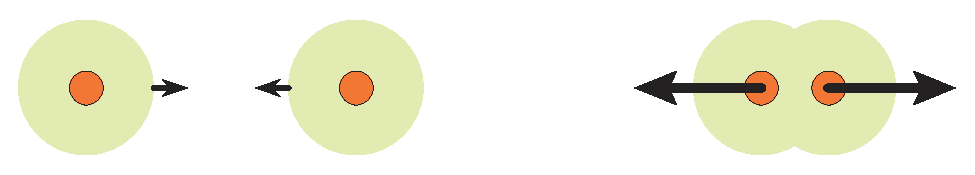
\includegraphics{GP011/GP011F05.eps}}
 \put(50,15){\makebox(0,0)[t]{\parbox{55mm}{
 Слабое притяжение нейтральных молекул
 }}}
 \put(145,15){\makebox(0,0)[t]{\parbox{58mm}{
 Сильное отталкивание положительных ядер
 }}}
 \end{picture}\\
 \begin{picture}(190,110)(0,0)
 %\put(0,0){\framebox(190,110)[b]{}}
 \put(0,0){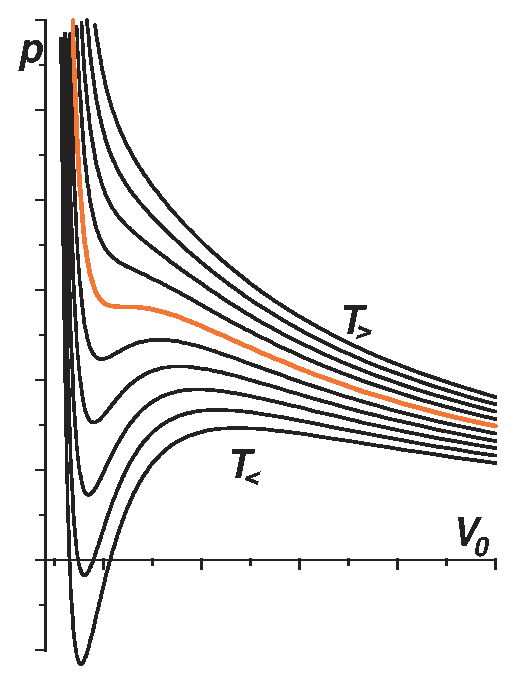
\includegraphics{GP011/GP011F06.eps}}
 \put(50,110){\makebox(0,0)[tl]{\parbox{140mm}{
 Уравнение состояния газа Ван-дер-Ваальса
 \begin{displaymath}
\left(p+\frac{a}{V_0^2}\right)\left(V_0-b\right)=RT
\end{displaymath}
  }}}
 \put(90,83){\makebox(0,0)[tl]{\parbox{100mm}{
 -- это уравнение 3 степени относительно $V_0$ при постоянных $p$ и $T$. Оно должно иметь 3 решения: при $T<T_k$ -- все вещественные, при $T>T_k$ -- одно вещественное и два комплексных.\\

 При большой $T$ кривая $p(V_0)$ ведет себя как изотерма для идеального газа, соответствующая закону Бойля-Мариотта $\left( pV_0={\rm const.}\right)$, а при малой...
  }}}
 \end{picture}\\
 \begin{picture}(190,110)(0,0)
 %\put(0,0){\framebox(190,110)[b]{}}
 \put(0,0){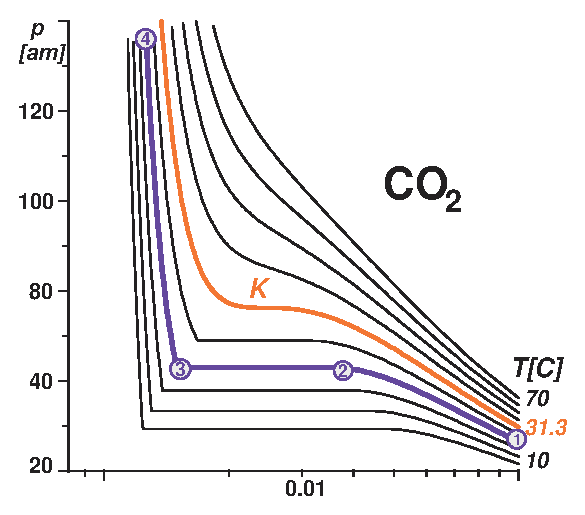
\includegraphics{GP011/GP011F07.eps}}
 \put(135,40){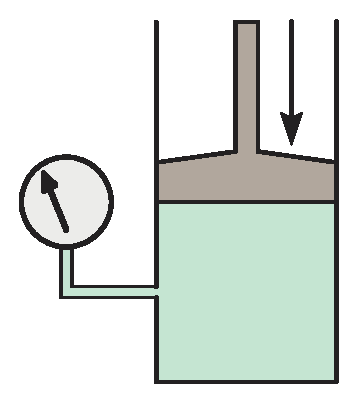
\includegraphics{GP011/GP011F08.eps}}
 \put(20,110){\makebox(0,0)[tl]{\parbox{130mm}{
Будем сжимать газ CO$_2$, поддерживая его температуру постоянной, и записывать величину давления при разном объеме.
  }}}
 \put(190,0){\makebox(0,0)[br]{\parbox{85mm}{
участок (1---2): давление растет.\\
участок (2---3): газ сжижается, давление остается постоянным.\\
участок (3---4): сжатие жидкости.
  }}}
 \end{picture}\\

 Давление, при котором происходит сжижение, -- {\bf упругость на\-сы\-щен\-ных паров при данной температуре}.
 
 %\newpage
 \noindent
 \begin{picture}(190,105)(0,0)
 %\put(0,0){\framebox(190,105)[b]{}}
 \put(0,0){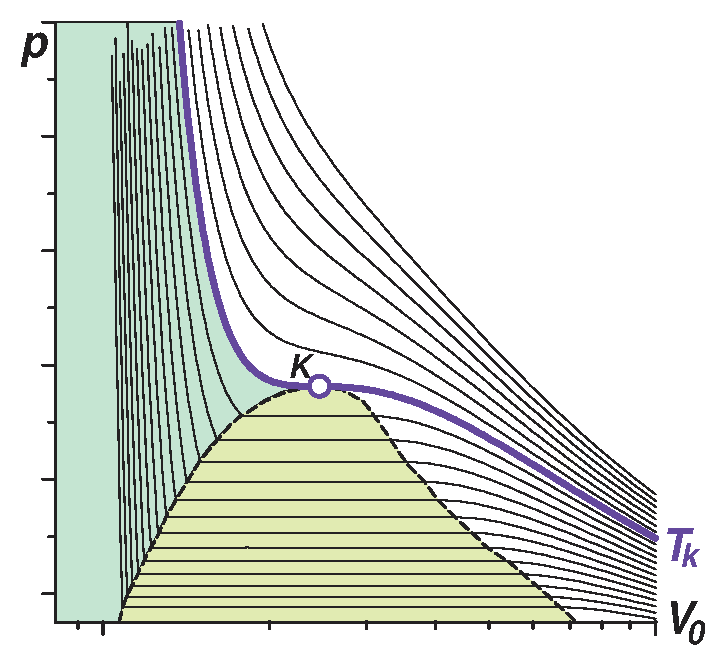
\includegraphics{GP011/GP011F09.eps}}
 \put(60,106){\makebox(0,0)[tl]{\parbox{130mm}{
 Если температура выше критической, то сжижение невозможно. Изотерма, которая отделяет семейство изотерм с провалом от семейства изотерм без провала, -- {\bf критическая изотерма}.
  }}}
 \put(120,75){\makebox(0,0)[tl]{\parbox{70mm}{
 При температуре ниже кри\-тической вещество мо\-жет существовать либо как газ, либо как жидкость, либо как и жид\-кость и на\-сы\-щен\-ный пар од\-но\-вре\-мен\-но (в зависимости от давления). Для воды, e.g., $T_k=374^\circ$C.
 Упругость насыщенного па\-ра $\leq p_k$ (критическое дав-
  }}}
 \end{picture}\\
ление). Объем жидкости $\leq V_k$ (критический объем). В критической точке пропадает всякое различие между жидкостью и газом.

При $p<p_0$ (давления насыщенного пара) можно получить жидкость в ($\bullet$){\bf A} без ее перехода в газ (растянутая жидкость). Аналогично, при $p>p_0$ можно получить газ в ($\bullet$){\bf B} без его конденсации (пересыщенный пар).\\
 \begin{picture}(190,100)(0,0)
 %\put(0,0){\framebox(190,100)[b]{}}
 \put(0,0){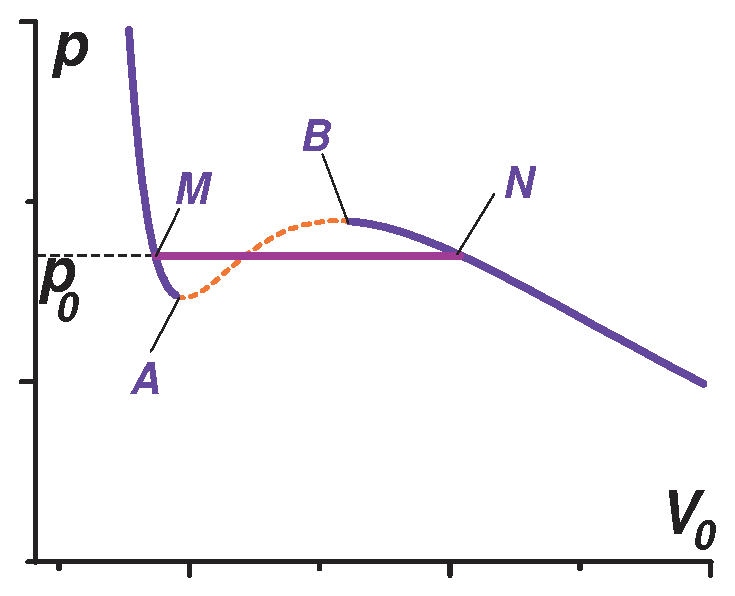
\includegraphics{GP011/GP011F10.eps}}
 \put(110,98){\makebox(0,0)[tl]{\parbox{80mm}{
 Оба эти состояния очень не\-устойчивы. При появлении малейшей ``провокации'' рас\-тя\-ну\-тая жидкость закипает, а пере\-сы\-щен\-ный пар кон\-ден\-си\-ру\-ет\-ся (вспомните иммерсион\-ный след за самолетом).
  }}}
 \put(125,44){\makebox(0,0)[tl]{\parbox{65mm}{
  Первое явление использу\-ет\-ся для регистрации субатомных частиц в пузырьковой камере, а второе -- в камере Вильсона.
  }}}
 \end{picture}\\
\underline{\bf Внутренняя энергия реального газа.}

Как ранее говорилось, для \underline{идеального газа} внутренняя энергия $U$ -- это кинетическая энергия движения молекул:
\begin{displaymath}
U = E_k=\sum\overline{w}_k = C_V\;T
\end{displaymath}
Она не зависит ни от давления, ни от объема, а только от температуры и вида молекул.

В \underline{реальном} же газе $\exists$ силы между молекулами (и притяжение, и отталкивание) $\Rightarrow$ кроме кинетической $\exists$ еще и потенциальная энергия
\begin{displaymath}
U = E_k + E_p
\end{displaymath}
 \begin{picture}(185,80)(0,0)
 %\put(0,0){\framebox(185,75)[b]{}}
 \put(15,0){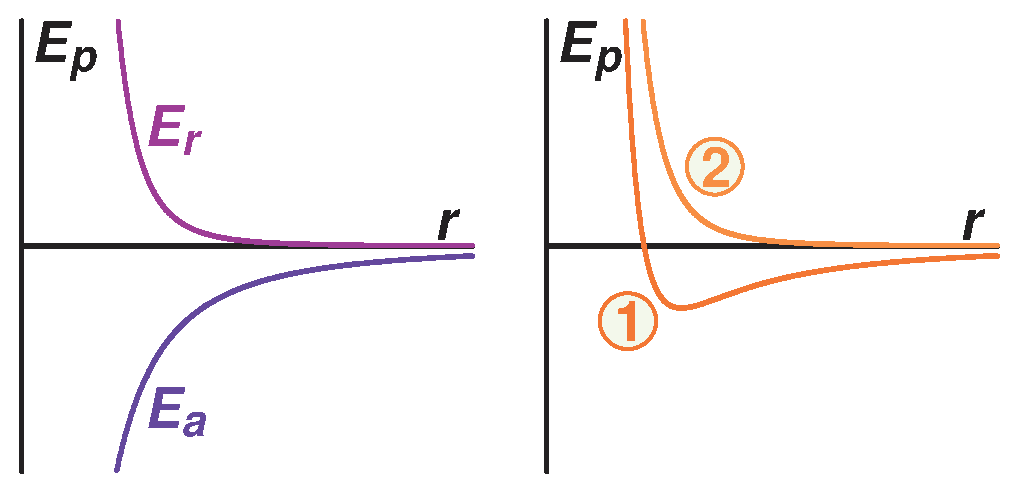
\includegraphics{GP011/GP011F11.eps}}
 \put(0,38){\makebox(0,0)[tl]{\parbox{50mm}{
 }}}
 \end{picture}\\
Как мы видели, $E_p$ зависит от расстояния между молекулами $\Rightarrow$ зависит от объема $V$.

Если объем увеличить (без совершения внешней работы), то притяже\-ние ослабнет, потенциаль\-ная энергия слегка возрастет, а кинетической придется уменьшится (чтобы полная энергия не изменилась). Иначе говоря, при удалении молекул друг от друга притяжение их слегка притормаживает. В итоге, скорость молекул упадет $\Rightarrow$ температура тоже упадет!

Btw, еще не факт, кто ``побеждает'' на больших расстояниях -- притяже\-ние (результирующая кривая 1) или отталкивание (кривая 2)... Если оттал\-ки\-ва\-ние -- то при расширении газа скорость (и температура) только увели\-чит\-ся.

 Джеймс Джоуль пытался в конце IXX века это обнаружить. Удалось позднее, когда они вместе с Вильямом Томсоном заменили кран на пористую пробку ({\bf дросселирование})\\ \begin{picture}(185,110)(0,0)
 %\put(0,0){\framebox(185,75)[b]{}}
 \put(10,0){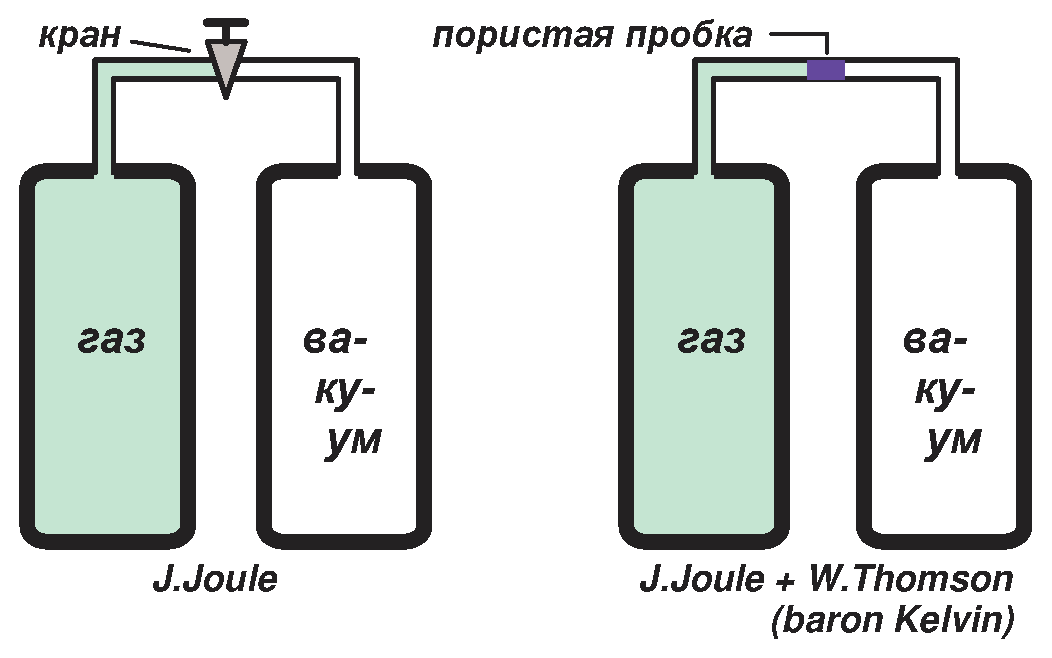
\includegraphics{GP011/GP011F12.eps}}
 \put(0,38){\makebox(0,0)[tl]{\parbox{50mm}{
 }}}
 \end{picture}\\
Большинство газов остывало (положительный эффект Джоуля-Томсона). Но некоторые (водород) -- нагревались (отрицательный эффект Джоуля-Томсона).

Это зависит от того, которая из поправок Ван-дер-Ваальса больше -- ответственная за притяжение ($a$) или за отталкивание ($b$). Один и тот же газ может иметь разный знак эффекта Дж-Т при разных условиях. При больших давлениях размеры молекул важнее $\Rightarrow$ отталкивание переве\-ши\-ва\-ет $\Rightarrow$ эффект Дж-Т = --- (нагревание).\\

\underline{\bf Ожижение газов.}
\begin{center}
\begin{tabular}{|c||c|c|c|c|c|c|c|c|c|}\hline
Вещество                 & H$_2$O & CO$_2$ & Kr & O$_2$ & Ar & N$_2$ & Ne & H$_2$ & He  \\ \hline \hline
 $T_k \;\;[^\circ\rm C]$ & 374 & 31 & --62.5 & --118.8 & --122.4 & --147 & --228 & --240 & --267.9 \\ \hline
 $p_k \;\;[\rm am]$      & 217 & 73 & 54 & 50 & 48 & 33.5 & 26 & 12.85 & 2.2 \\ \hline
\end{tabular}
\end{center}
Видим, что для ожижения одного только сжатия мало. Надо и охлаждать.

%\newpage
\noindent
Пикт\'{е} (Raoul Pictet, 1877, Geneva): предварительное охлаждение за счет интенсивного испарения.
\begin{enumerate}
\item Жидкий сернистый ангидрид испаряется $\Rightarrow$ охлаждается.
\item В нем по змеевику охлаждается CO$_2$, а затем сжимается и ожижается.
\item Жидкая CO$_2$ интенсивно испаряется $\Rightarrow$ охлаждается до --130$^\circ$С.
\item В нем по змеевику охлаждается сжатый O$_2$, а затем сжимается еще сильнее и ожижается.
\end{enumerate}
В 1884 г. З.Вроблевский и К.Ольшевский (1884, Krakow) этим кипящим O$_2$ охладили H$_2$ и при p=190 ат сжижили его.\\
Использование (+)-эффекта Джоуля-Томсона: {\bf цикл Хэмпсона--Линде}.
(Carl Paul Gottfried von Linde, M\"{u}nchen, 1895)

Газ многократно сжимается $\Rightarrow$ нагревается, затем это выделившееся тепло у него отбирается в теплообменнике. Потом газ расширяется $\Rightarrow$ охлаждается. Этот холод используется для предварительного охлаждения следующей порции газа перед его расширением. Будучи сначала охлаж\-ден\-ным, он потом еще и расширяется $\Rightarrow$ охлаждается еще сильнее. Этот ``удвоенный'' холод идет на предварительное охлаждение третьей порции газа перед его расширением. И так далее.

Heike Kamerlingh Onnes (Leiden, NL) получил в 1908 г. жидкий гелий (предварительно охладив его кипящим жидким водородом) при 4.22~К и Нобелевскую Премию (1913).

Можно отбирать у сжатого газа внутреннюю энергию за счет совер\-ше\-ния им работы против внешних сил (чтобы газ, расширяясь, двигал поршень или крутил турбину).

Зачем нужен жидкий газ? Кроме чисто исследовательского интереса, есть и прикладное значение. Жидкий газ сохраняет свою температуру $T_{\texttt{кипения}}$ до тех пор, пока весь не выкипит $\Rightarrow$ можно с его помощью ``транспортировать холод''.

Сверхнизкие температуры (4 мК) удается получить при растворении одного жидкого газа в другом ($^3$He в $^4$He). Сначала их оба охлаждают от 4.4 до 0.7 К, заставляя быстро испаряться, а потом сливают вместе.
